\documentclass{beamer}
\usepackage{graphicx}
\usepackage{animate}
\usepackage{textcomp}
\usepackage{multimedia}
\usetheme{Warsaw}


\title[]{EE1390}
\subtitle{Prototype methods}
\author{EE18BTECH11025 and EE18BTECH11016}
\date{}

\begin{document}


\begin{frame}
\titlepage
\end{frame}

\begin{frame}{Prototype Methods}
A prototype is an element of the data space that represents a group of elements.

A cluster prototype serves to characterize the cluster, their elements.


\end{frame}

\begin{frame}{ K-means Clustering}
K-means clustering is a method for finding clusters and cluster centers in a set of unlabeled data.

 One chooses the desired number of cluster centers, say R, and the K-means procedure iteratively moves the centers to minimize the total within cluster variance.
 \end{frame}
 
 \begin{frame}{ K-means Clustering}
 Given an initial set of centers, the K-means algorithm alternates the two steps:

  1. for each center we identify the subset of training points (its cluster)that is closer to it than any other center
  
  
  2. the means of each feature for the data points in each cluster are computed, and this mean vector becomes the new center for that cluster
 
\end{frame}


\begin{frame}
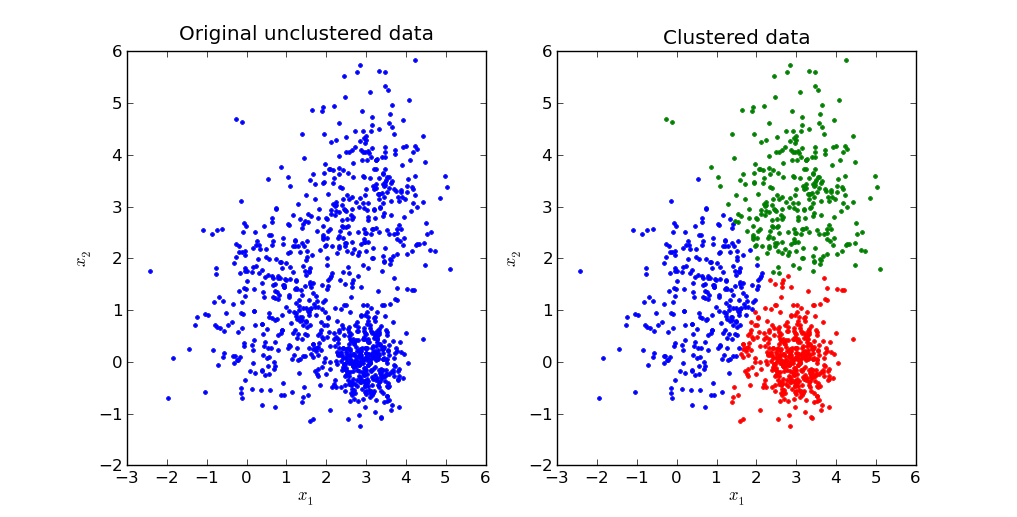
\includegraphics[scale=.3]{1.png}  
\end{frame}


\begin{frame}
\centering
    \movie[loop,width=\textwidth]{
        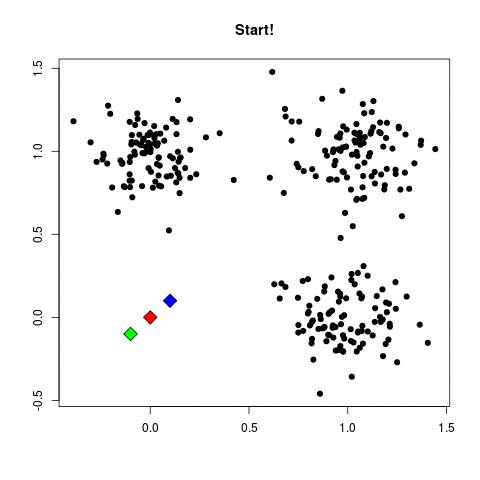
\includegraphics[scale=0.5]{l.png}
    }{l.wmv}

\end{frame}

\begin{frame}{Linear Vector Quantization}
Prototypes are placed strategically with respect to the decision boundaries in an ad-hoc way. LVQ is an online algorithm, observations are processed one at a time.


The idea is that the training points attract prototypes of the correct class,and repel other prototypes.

 When the iterations settle down, prototypes should be close to the training points in their class. 
 
 The learning rate $\alpha$ is decreased to zero with each iteration
\end{frame}

\begin{frame}{Linear Vector Quantization}
1. Choose R initial prototypes for each class: $m_1$(k), $m_2$(k), . . . , $m_R$(k), k= 1,2, . . . , K, for example, by sampling R training points at random from each class.

\vspace{2 mm}
2. Sample a training point $x_i$ randomly (with replacement), and let (j, k)index the closest prototype $m_j$(k) to $x_i$

\vspace{2 mm}
\setlength{\parindent}{0.5cm}(a) If $g_i$ = k(i.e., they are in the same class), move the 

\ \ \ \ \ prototype towards the training point:
 \setlength{\parindent}{1.5cm}
 \vspace{2 mm}
 
 $m_j$(k)  \textleftarrow{}  $m_j$(k) + $\alpha$($x_i$ - $m_j$(k)),
 
 \vspace{2 mm}
 where $\alpha$ is the learning rate.
 
 \vspace{2 mm}
\setlength{\parindent}{0.5cm}


(b) If $g_i$ $\neq$ k (i.e., they are in different classes), move the


 prototype away from the training point:

 \vspace{2 mm}
\setlength{\parindent}{1.5cm}
 $m_j$(k)  \textleftarrow{}  $m_j$(k) - $\alpha$($x_i$ - $m_j$(k))
\setlength{\parindent}{0cm}

\vspace{2 mm}
3. Repeat step 2, decreasing the learning rate with each iteration towards zero.

\end{frame}


\begin{frame}
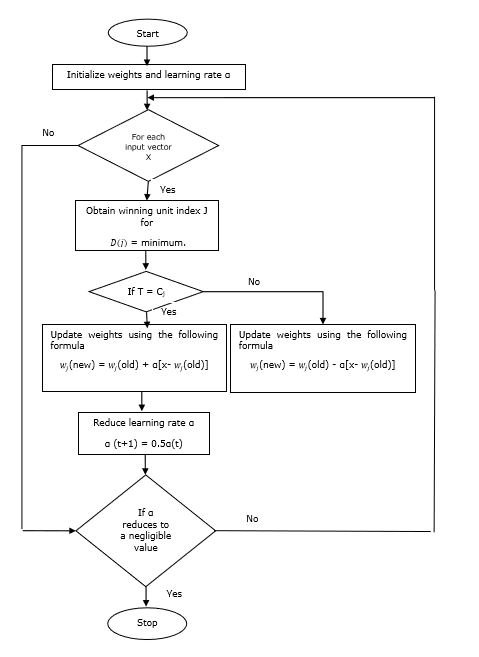
\includegraphics[scale=0.5]{flowchart.png} 
\end{frame}

\begin{frame}{LVQ2}
The condition of LVQ2 is formed by window. This window will be based on the following parameters:

    x - the current input vector

    yc - the reference vector closest to x

    yr - the other reference vector, which is next closest to x

    dc - the distance from x to yc

    dr - the distance from x to yr
    
    
    \vspace{2 mm}

The input vector x falls in the window, if:
\setlength{\parindent}{2cm}


$d_c$/$d_r$ $>$ 1 - $\theta$   and    $d_r$/$d_c$ $>$ 1 + $\theta$

Here, $\theta$ is the number of training samples.
\end{frame}

\begin{frame}
Updating can be done with the following formula 

 \vspace{2 mm}
$y_c$(t+1)=$y_c$(t)+α(t)[x(t) - $y_c$(t)]   \ \ \ \ \ \ (belongs to different class)

 \vspace{2 mm}
$y_r$(t+1)=$y_r$(t)+α(t)[x(t) - $y_r$(t)]   \ \ \ \ \ \ (belongs to same class)

 \vspace{2 mm}
Here $\alpha$ is the learning rate.
\end{frame}

\begin{frame}{LVQ3}
In LVQ3, we will take the two closest vectors namely $y_c1$ and $y_c2$ and the condition for window is as follows −
 \vspace{2 mm}
 
Min[$d_c1$/$d_c2$, $d_c2$/$d_c1$]$>$(1 - $\theta$)(1 + $\theta$)
 \vspace{2 mm}
 
Here $\theta$ $\approx$ 0.2

 \vspace{2 mm}
Updating can be done with the following formula −

 \vspace{2 mm}
$y_c1$(t+1)=$y_c1$(t) + $\beta$(t)[x(t) - $y_c1$(t)]       \ \ \ \ \ \ (belongs to different class)



 \vspace{2 mm}
$y_c2$(t+1)=$y_c2$(t) + $\beta$(t)[x(t) - $y_c2$(t)]          \ \ \ \ \ \ (belongs to same class)



 \vspace{2 mm}
Here $\beta$
is the multiple of the learning rate $\alpha$ and $\beta$ = m$\alpha$(t) for every 0.1 $<$ m $<$ 0.5
\end{frame}
\end{document} 

  
  